\section{Pickling and Unpickling}
This section explains how pickling and unpickling is organized.
\subsection{Design Goals}
Pickling and unpickling services are designed to
\begin{itemize}
\item work for all resource free store datastructures.
\item preserve sharing and cycles.
\item operate language independently.
The pickler and unpickler only operate on store level.
They do not know anything about language specific datatypes.
\item operate as a concurrent operation.
Pickling and unpickling are handled like all other concurrent computations.
In particular, they might be preempted.

The pickler and unpickler are eager.
They automatically request transients.
\end{itemize}
\subsection{Model}
\begin{figure}[ht]
\centering
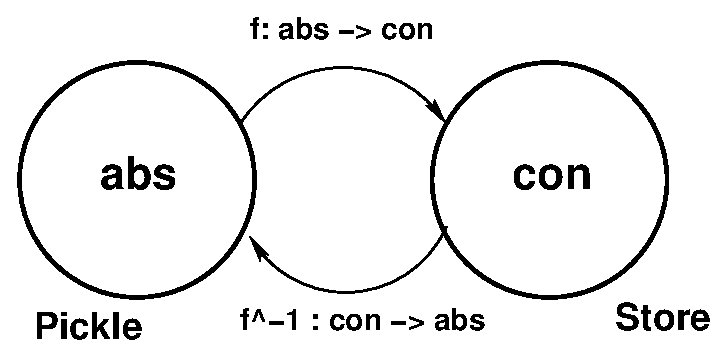
\includegraphics[width=5cm]{figures/pickler_model.eps}
\caption{\label{model_pickler} {\it Pickling model}}
\end{figure}
Let $\text{con}$ be the set of all resource free store datatructures
and $\text{abs} \subseteq \text{con}$
be the set of all abstract representations created by the transfer language.

Pickling and unpickling are
defined with resepect to a bijective import function
$f : \text{abs} \rightarrow \text{con}$ as shown in figure \ref{model_pickler}.

The key idea is that the unpickler applies this function to the
previously unpickled abstract representation of the value.

The pickler on the other hand
applies the inverse function to the value to be pickled
and pickles the regained abstract representation.
\begin{paragraph}{Pointwise definition.}
The machine supports the plug-in of new interpreters during runtime.
To cope with this, the function $f$ is defined
pointwise using triples $(id, c, a)$ where $id$
is a globally unique identifier.

The machine starts with a trivial definition of $f$, namely the identity
function. As computation proceeds, $f$ is pointwise refined.
\end{paragraph}
\begin{paragraph}{Modelling Primitives.}
The transfer language provides a mechanism called transforms to express
$id: f(a) = c$. Transforms are discussed in section \ref{transform_sect}.

The inverse mechanism is a special store block called BlockWithHandler.
It is used to express $id: f^{-1}(c) = a$.
BlockWithHandler are discussed in section \ref{blockhandler_sect}.
\end{paragraph}
\subsection{Transforms}
\label{transform_sect}
A {\em transform} is a globally unique identifier naming a
mapping together with the argument of the mapping.
This argument is the abstract representation created by the transfer
language.

The pickler and unpickler are parameterized over a transform table
mapping the identifier to the corresponding map function.
\begin{paragraph}{Applying transforms.}
Every time the unpickler reads such a tranform it first reads
the identifier and the corresponding externalized representation
of the argument.

The unpickler then tries to lookup
the corresponding mapping in the transform table of the site the unpickler
runs on using the read identifier.

In case the lookup fails, an exception is raised.

In case the lookup succeeds, the obtained mapping is applied to the external
representation.
Its result is wrapped into a BlockWithHandler which itself
is linked into the created graph.
\end{paragraph}
\subsection{BlockWithHandler}
\label{blockhandler_sect}
A BlockWithHandler is a normal store block, with a a handler added
that delivers the abstract representation of the previous performed
transform again.

The language provider is given the choice to either compute
this representation using a inverse function or simply retrieve
the encapsulated (by closing over it) original version.

Each time the pickler runs into a block with handler,
it executes this handler and pickles the resulting
abstract representation.
\subsection{Transfer Language}
\begin{figure}[ht]
\begin{verbatim}
pickle    ::= int | chunk | block | tuple | closure | transform
int       ::= POSINT <uint> | NEGINT <uint>
chunk     ::= CHUNK size <byte>*size
size      ::= <uint>
block     ::= BLOCK label size field*size
tuple     ::= TUPLE size field*size
closure   ::= CLOSURE size field*size
label     ::= <uint>
field     ::= pickle | reference
reference ::= REF id
id        ::= <uint>
transform ::= TRANSFORM (chunk|reference) field
\end{verbatim}
\caption{\label{pickle_lang} {\it Pickle format}}
\end{figure}
Figure \ref{pickle_lang} shows a EBNF like grammar of the transfer
language. 
